\documentclass{article}
\usepackage[russian]{babel}
\usepackage[utf8]{inputenc}
\usepackage{amsfonts}
\usepackage{amssymb}
\usepackage{listings}
\usepackage{amsmath}
\usepackage{amsthm}
\usepackage{minted}
\usepackage{indentfirst}
\usepackage{hyperref}
\usepackage{cleveref}
\usepackage{graphicx}
\usepackage{wrapfig}
\usepackage{tikz}
\usepackage{ragged2e}
\usepackage{multirow}

\title{СМВМ, задание №1.}
\author{Болохонов Артем Владимирович}

\begin{document}

\date{}
\maketitle

\begin{center}
    {\section*{Основное задание}}
\end{center}


\textbf{Описание задания:} в качестве базиса полиномиального пространства использовались мономы, для реализации \textit{QR}-алгоритма использовался метод вращений с
выбором главного элемента. Программа написана на языке Python.


Расчеты проводились на компьютере AMD Ryzen 7 7700x 4.5GHz (up to 5.4 GHz), 8 cores; DIMM DDR5 32 Gb 6000 MHz.


В качестве решателя системы в \textit{методе нормальных уравнений} использовалась функция \texttt{linalg.solve} из библиотеки \texttt{numpy}. Это является возможной причиной более быстрого решения системы в случае использования данного алгоритма.

Далее идут таблицы с результатами вычислений на различных файлах.

\begin{table}[h!]
\begin{tabular}{|l||l|l|l||l|l|l|}
\hline
N & $cond_2(A)$ & t (sec)    & NRMSE    & $cond_2(A^TA)$ & t (sec)    & NRMSE    \\ \hline
0 & 1.00e+00   & 4.4209e-02 & 2.88e-01 & 1.00e+00                       & 3.0005e-03 & 2.88e-01 \\ \hline
1 & 1.75e+01   & 8.1009e-02 & 1.14e-02 & 3.06e+02                       & 3.0005e-03 & 1.14e-02 \\ \hline
2 & 3.41e+02   & 1.1717e-01 & 6.72e-04 & 1.16e+05                       & 6.0005e-03 & 6.72e-04 \\ \hline
3 & 6.83e+03   & 1.5568e-01 & 6.69e-04 & 4.67e+07                       & 5.0013e-03 & 6.69e-04 \\ \hline
4 & 1.39e+05   & 1.8417e-01 & 6.66e-04 & 1.94e+10                       & 6.0015e-03 & 6.66e-04 \\ \hline
5 & 2.87e+06   & 1.8855e-01 & 5.40e-04 & 8.24e+12                       & 7.0014e-03 & 4.41e-04 \\ \hline
6 & 5.95e+07   & 1.9106e-01 & 5.00e-03 & 3.54e+15                       & 7.1044e-03 & 2.47e-04 \\ \hline
7 & 1.24e+09   & 1.9316e-01 & 9.81e-03 & 1.54e+18                       & 8.6784e-03 & 2.36e-04 \\ \hline
8 & 2.61e+10   & 1.9600e-01 & 1.04e-02 & 6.81e+20                       & 8.8663e-03 & 2.03e-04 \\ \hline
9 & 5.51e+11   & 2.0879e-01 & 1.06e-02 & 3.03e+23                       & 1.1000e-02 & 1.80e-04 \\ \hline
\end{tabular}
\caption{результаты вычислений на файле \texttt{data\_2.txt}.}
\end{table}

\begin{table}[H]
\begin{tabular}{|l||l|l|l||l|l|l|}
\hline
N & $cond_2(A)$ & t (sec)    & NRMSE    & $cond_2(A^TA)$ & t (sec)    & NRMSE    \\ \hline
0 & 1.00e+00   & 8.0023e-03 & 3.32e-01 & 1.00e+00                       & 1.0056e-03 & 3.32e-01 \\ \hline
1 & 4.39e+00   & 1.5143e-02 & 8.30e-02 & 1.92e+01                       & 1.0002e-03 & 8.30e-02 \\ \hline
2 & 2.28e+01   & 2.3132e-02 & 1.43e-15 & 5.22e+02                       & 1.0002e-03 & 6.73e-15 \\ \hline
3 & 1.24e+02   & 2.9006e-02 & 1.90e-15 & 1.54e+04                       & 9.9993e-04 & 2.57e-14 \\ \hline
4 & 6.88e+02   & 3.7009e-02 & 2.87e-15 & 4.73e+05                       & 1.0004e-03 & 9.43e-14 \\ \hline
5 & 3.85e+03   & 4.4004e-02 & 2.70e-15 & 1.48e+07                       & 2.0001e-03 & 2.98e-13 \\ \hline
6 & 2.17e+04   & 4.9999e-02 & 1.07e-15 & 4.70e+08                       & 2.0003e-03 & 6.18e-13 \\ \hline
7 & 1.23e+05   & 5.5015e-02 & 1.80e-15 & 1.51e+10                       & 1.0006e-03 & 4.32e-12 \\ \hline
8 & 6.97e+05   & 6.3044e-02 & 1.98e-15 & 4.86e+11                       & 2.0003e-03 & 5.22e-11 \\ \hline
9 & 3.97e+06   & 6.9114e-02 & 1.35e-15 & 1.58e+13                       & 2.1424e-03 & 3.04e-10 \\ \hline
\end{tabular}
\caption{результаты вычислений на файле \texttt{data\_4.txt}.}
\end{table}

\begin{table}[h!]
\begin{tabular}{|l||l|l|l||l|l|l|}
\hline
N & $cond_2(A)$ & t (sec)    & NRMSE    & $cond_2(A^TA)$ & t (sec)    & NRMSE    \\ \hline
0 & 1.00e+00   & 7.9992e-03 & 2.94e-01 & 1.00e+00                       & 0.0000e+00 & 2.94e-01 \\ \hline
1 & 4.39e+00   & 1.5749e-02 & 2.76e-02 & 1.92e+01                       & 0.0000e+00 & 2.76e-02 \\ \hline
2 & 2.28e+01   & 2.2108e-02 & 2.32e-03 & 5.22e+02                       & 1.0002e-03 & 2.32e-03 \\ \hline
3 & 1.24e+02   & 3.0004e-02 & 1.46e-04 & 1.54e+04                       & 1.0002e-03 & 1.46e-04 \\ \hline
4 & 6.88e+02   & 3.6003e-02 & 7.32e-06 & 4.73e+05                       & 1.0004e-03 & 7.32e-06 \\ \hline
5 & 3.85e+03   & 4.5005e-02 & 3.06e-07 & 1.48e+07                       & 2.0006e-03 & 3.06e-07 \\ \hline
6 & 2.17e+04   & 4.9733e-02 & 1.09e-08 & 4.70e+08                       & 1.0006e-03 & 1.09e-08 \\ \hline
7 & 1.23e+05   & 5.6402e-02 & 3.43e-10 & 1.51e+10                       & 2.0006e-03 & 3.43e-10 \\ \hline
8 & 6.97e+05   & 6.8017e-02 & 3.79e-11 & 4.86e+11                       & 2.0003e-03 & 3.01e-11 \\ \hline
9 & 3.97e+06   & 6.7099e-02 & 5.45e-11 & 1.58e+13                       & 2.2211e-03 & 8.85e-11 \\ \hline
\end{tabular}
\caption{результаты вычислений на файле \texttt{data\_5.txt}.}
\end{table}

\begin{figure}[H]
  \centering
  \subfloat{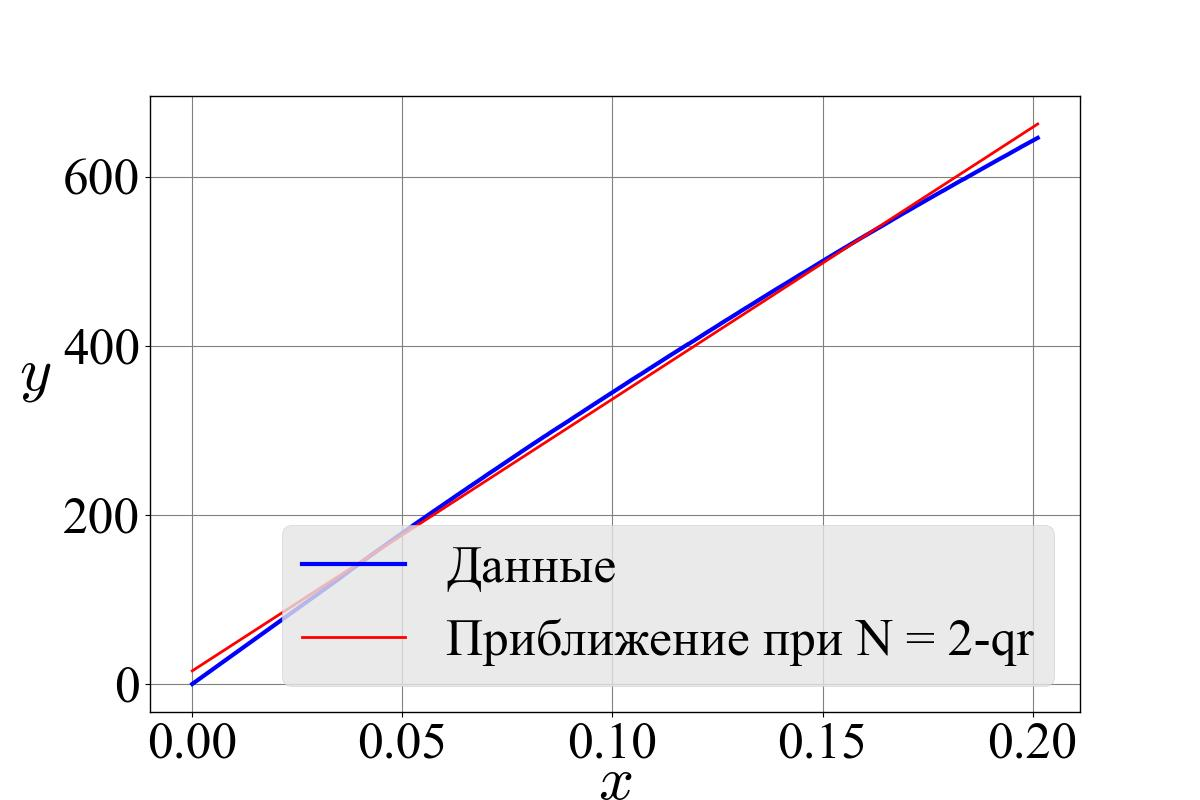
\includegraphics[width=0.45\textwidth]{data_2-qr-2.jpeg}}
  \hfill
  \subfloat{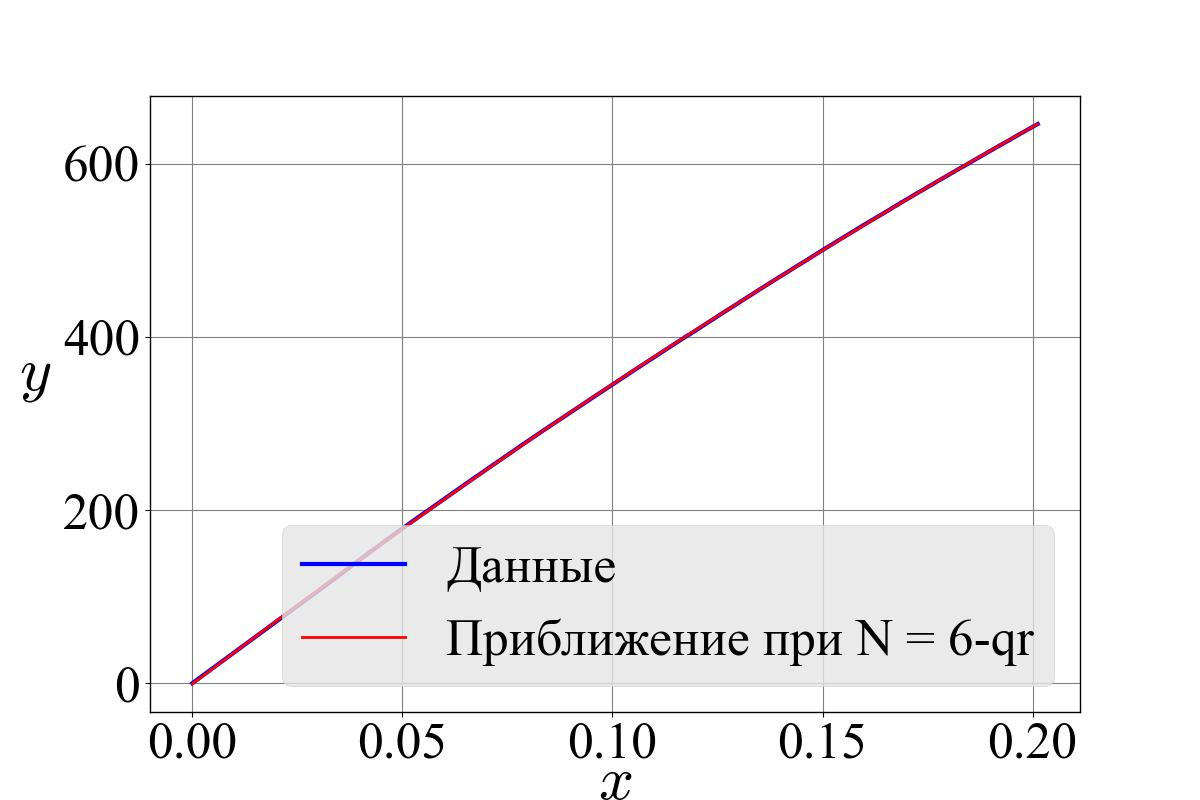
\includegraphics[width=0.45\textwidth]{data_2-qr-6.jpeg}}
  \caption{\centeringсравнение точного и приближенного решения на сетке с разбиением на входных данных \texttt{data\_2.txt} при $N = 2$ и $N = 5$.}
\end{figure}

Ответы на вопросы:
\begin{enumerate}
    \item \textit{Как отличаются числа обусловленности матриц при применении QR-алгоритма и метода НУ?} \\
    Число обусловленности при применении метода НУ квадратично больше, в сравнении с \textit{QR}-разложением. Это связано с тем, что в ходе вычислений, метод НУ взаимодействует с матрицей $A^TA$ (в \textit{QR}-методе просто $A$). Данную зависимость можно просмотреть на всех входных данных.
    \item \textit{Как убывает погрешность в зависимости от данных? Почему?} \\
    В целом можно наблюдать уменьшение погрешности на порядок при увеличении числа $N$ при использовании обоих методов. Тем не менее на входных данных \texttt{data\_2.txt} такой тенденции не наблюдается. Наоборот, при увеличении $N$, начиная с 6, \textit{QR}-алгоритм увеличивает погрешность вычислений. Это связано с тем, что данный набор данных представляет собой быстрые осцилляции, что и создает проблемы с вычислением.
    \item \textit{Как отличается погрешность при решении СЛАУ методом НУ и QR-алгоритмом?} \\
    Чисто теоретически \textit{QR}-алгоритм должен давать большую точность, т.к. работает с матрицами с меньшим числом обусловленности. На практике же не все так однозначно:
    \begin{itemize}
        \item \texttt{data\_2.txt}: метод НУ показывает себя стабильнее на шумных данных;
        \item \texttt{data\_4.txt}: \textit{QR}-метод быстрее достиг более высокой точности, чем метод нормальных уравнений;
        \item \texttt{data\_5.txt}: оба метода показывают плюс-минус одинаковую погрешность вычислений.
    \end{itemize}
\end{enumerate}
\end{document}
